
\section{Halbleiter}
\label{section:halbleiter}
\begin{frame}%STARTCONTENT
\begin{itemize}
  \item Weisen Eigenschaften von Leitern als auch von Nichtleitern auf
  \item Häufige Halbleiterelemente: Silizium oder Germanium
  \end{itemize}

\end{frame}

\begin{frame}
\frametitle{Diode}
\begin{columns}
    \begin{column}{0.48\textwidth}
    \begin{itemize}
  \item Einfachstes Halbleiter-Bauteil: Diode
  \item Strom kann nur in einer Richtung durch sie hindurchfließen
  \end{itemize}

    \end{column}
   \begin{column}{0.48\textwidth}
       
\begin{figure}
    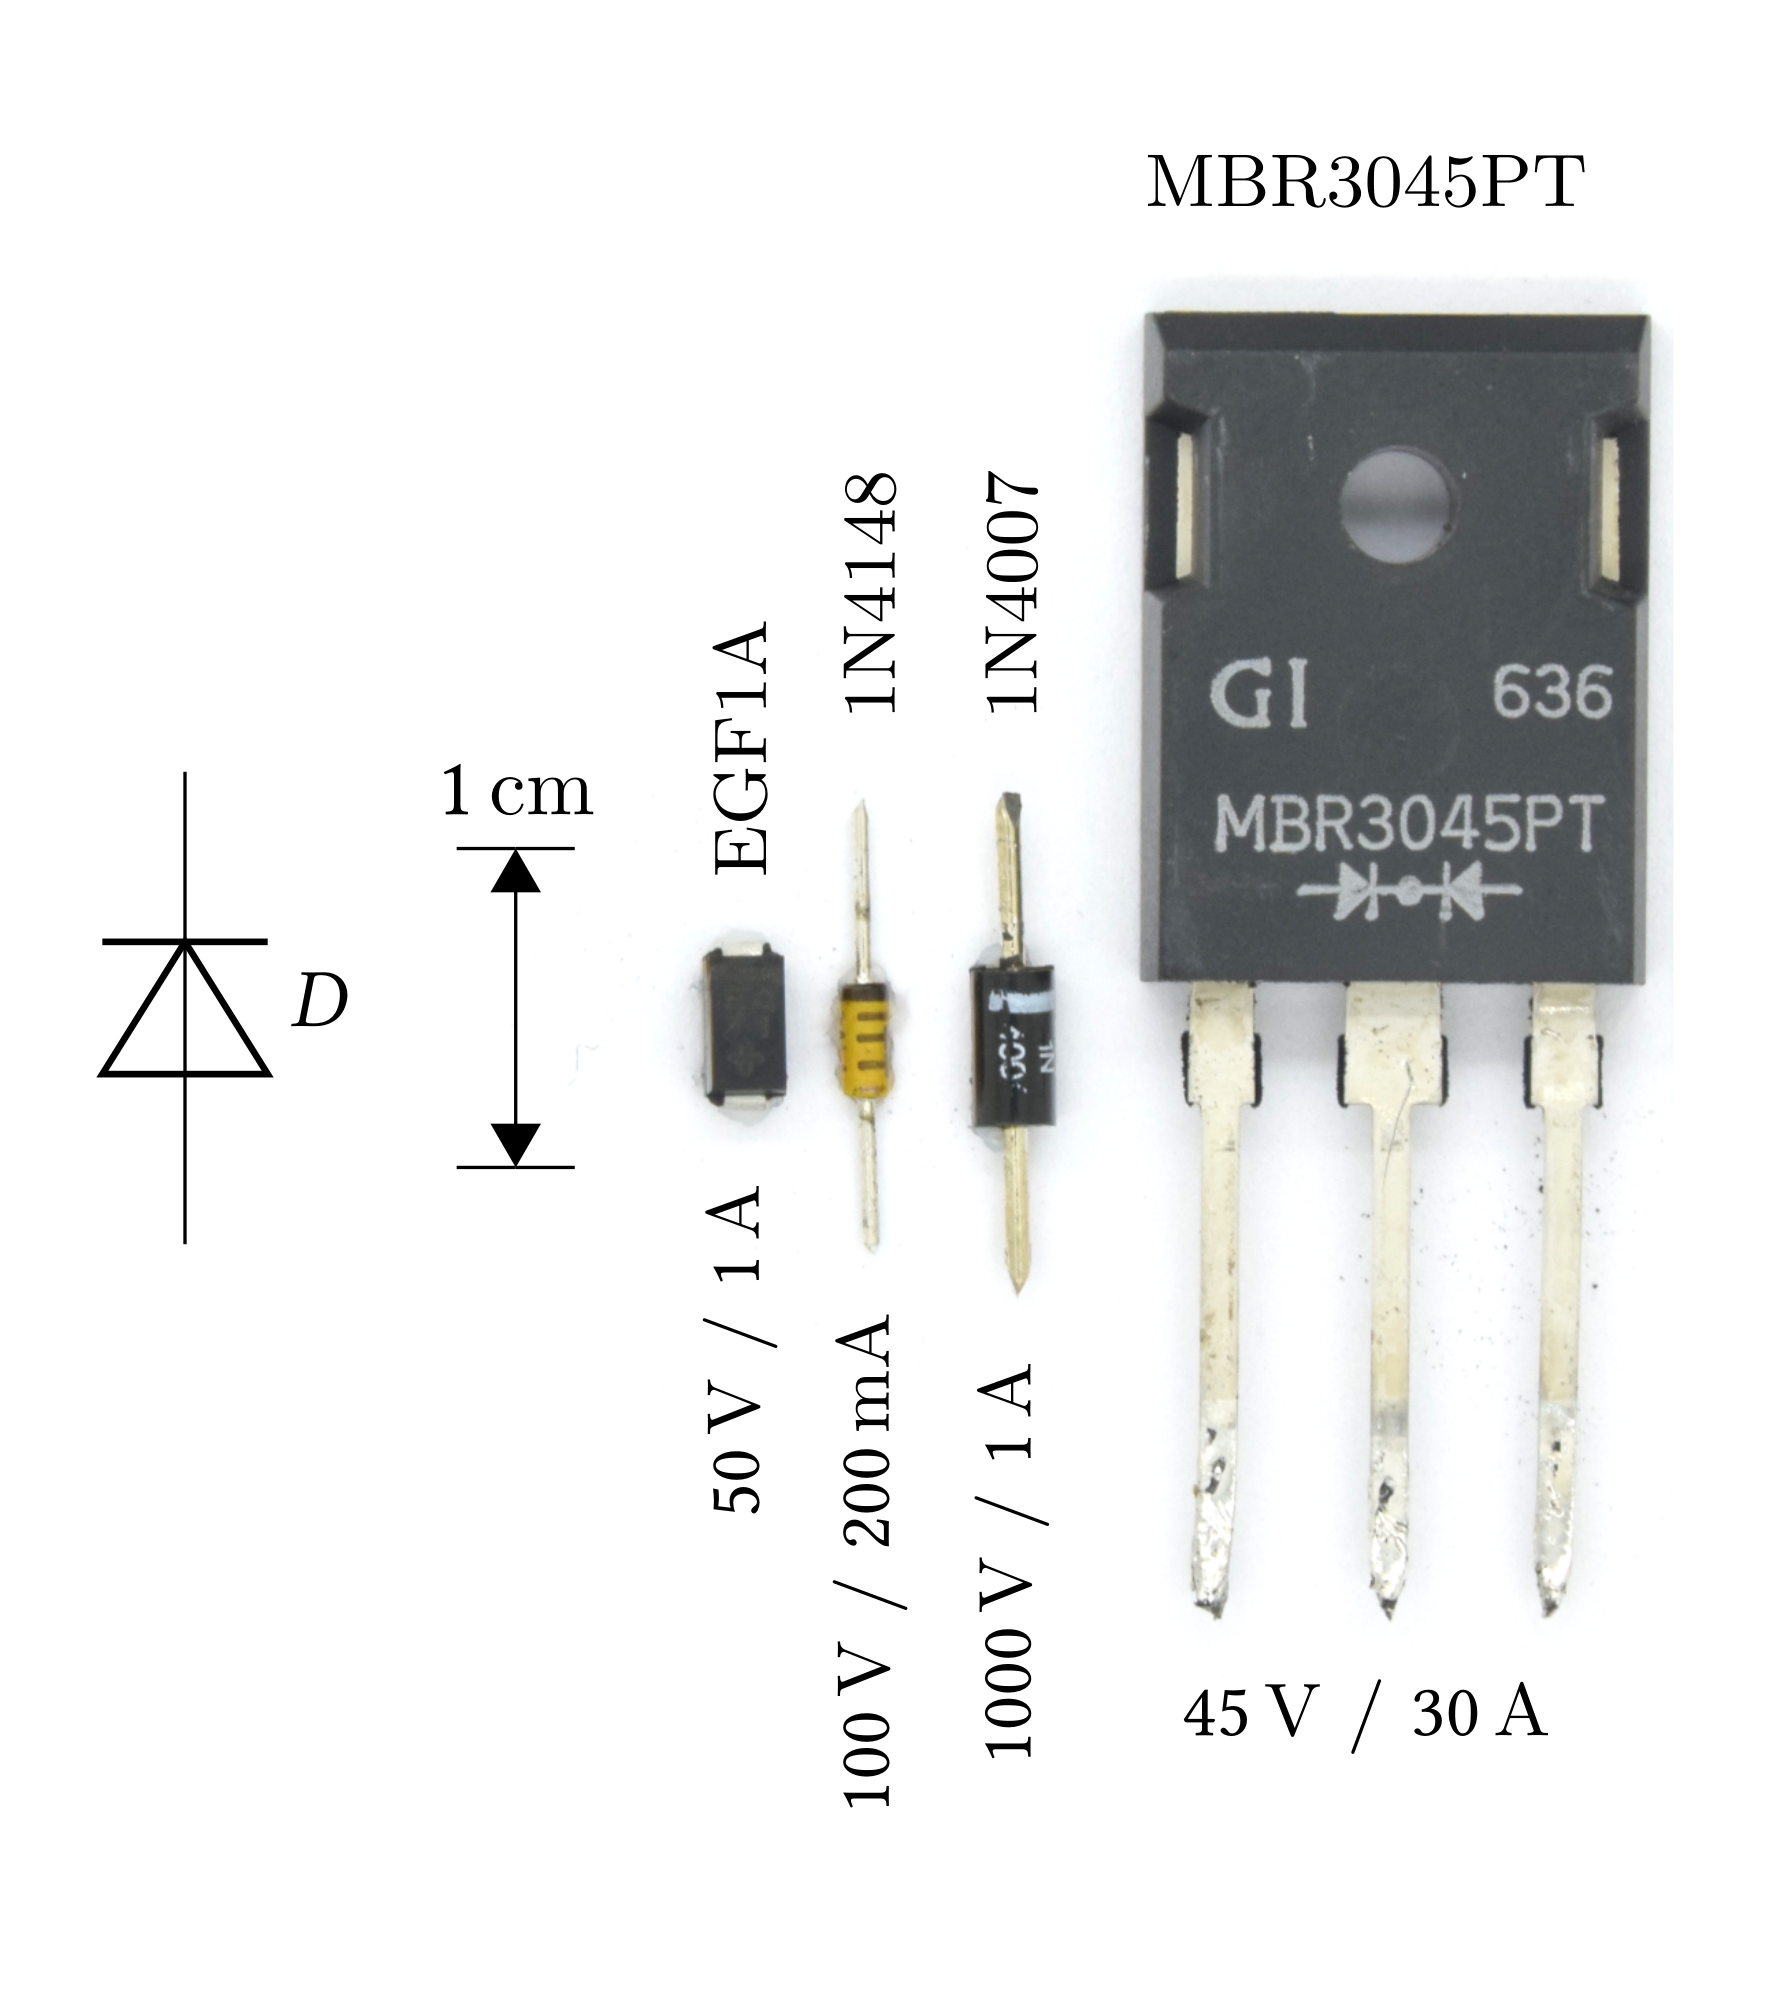
\includegraphics[width=0.85\textwidth]{foto/204}
    \caption{\scriptsize Schaltzeichen und Bauformen von Dioden}
    \label{n_halbleiter_dioden}
\end{figure}

   \end{column}
\end{columns}

\end{frame}

\begin{frame}
\only<1>{
\begin{PQuestion}{NC401}{Welches Bauteil wird durch das Schaltzeichen symbolisiert?}{Spule}
{Widerstand}
{Diode}
{Kondensator}
{\DARCimage{0.5\linewidth}{381include}}\end{PQuestion}

}
\only<2>{
\begin{PQuestion}{NC401}{Welches Bauteil wird durch das Schaltzeichen symbolisiert?}{Spule}
{Widerstand}
{\textbf{\textcolor{DARCgreen}{Diode}}}
{Kondensator}
{\DARCimage{0.5\linewidth}{381include}}\end{PQuestion}

}
\end{frame}

\begin{frame}
\frametitle{Anschlüsse einer Diode}
\begin{columns}
    \begin{column}{0.48\textwidth}
    \begin{itemize}
  \item Anode und Kathode
  \item Plus-Pol an Anode und Minus-Pol an Kathode: \emph{Diode leitet}
  \item Plus-Pol an Kathode und Minus-Pol an Anode: \emph{Diode sperrt}
  \end{itemize}

    \end{column}
   \begin{column}{0.48\textwidth}
       
\begin{figure}
    \DARCimage{0.85\linewidth}{666include}
    \caption{\scriptsize Merkhilfe Diode}
    \label{n_halbleiter_diode_merkhilfe}
\end{figure}


   \end{column}
\end{columns}

\end{frame}

\begin{frame}
\only<1>{
\begin{PQuestion}{NC403}{Wie lauten die Bezeichnungen für die Anschlüsse 1 und 2 im Schaltsymbol?}{1 = Anode; 2 = Kathode}
{1 = Kathode; 2 = Anode}
{1 = Basis; 2 = Kathode}
{1 = Emitter; 2 = Anode}
{\DARCimage{0.5\linewidth}{383include}}\end{PQuestion}

}
\only<2>{
\begin{PQuestion}{NC403}{Wie lauten die Bezeichnungen für die Anschlüsse 1 und 2 im Schaltsymbol?}{\textbf{\textcolor{DARCgreen}{1 = Anode; 2 = Kathode}}}
{1 = Kathode; 2 = Anode}
{1 = Basis; 2 = Kathode}
{1 = Emitter; 2 = Anode}
{\DARCimage{0.5\linewidth}{383include}}\end{PQuestion}

}
\end{frame}

\begin{frame}
\only<1>{
\begin{question2x2}{NC404}{In welchem der abgebildeten Stromkreise fließt Strom?}{\DARCimage{0.75\linewidth}{520include}}
{\DARCimage{0.75\linewidth}{519include}}
{\DARCimage{0.75\linewidth}{518include}}
{\DARCimage{0.75\linewidth}{521include}}
\end{question2x2}

}
\only<2>{
\begin{question2x2}{NC404}{In welchem der abgebildeten Stromkreise fließt Strom?}{\DARCimage{0.75\linewidth}{520include}}
{\DARCimage{0.75\linewidth}{519include}}
{\textbf{\textcolor{DARCgreen}{\DARCimage{0.75\linewidth}{518include}}}}
{\DARCimage{0.75\linewidth}{521include}}
\end{question2x2}

}
\end{frame}

\begin{frame}
\frametitle{LED}
\begin{columns}
    \begin{column}{0.48\textwidth}
    \begin{itemize}
  \item Leuchtdiode, \enquote{light-emitting diode}
  \item Leuchtet, sobald Strom durch sie hindurchfließt
  \item Schaltbild: Diode mit zwei zusätzlichen Pfeilen nach außen
  \item Verhält sich wie Diode, aber leuchtet
  \end{itemize}

    \end{column}
   \begin{column}{0.48\textwidth}
       
\begin{figure}
    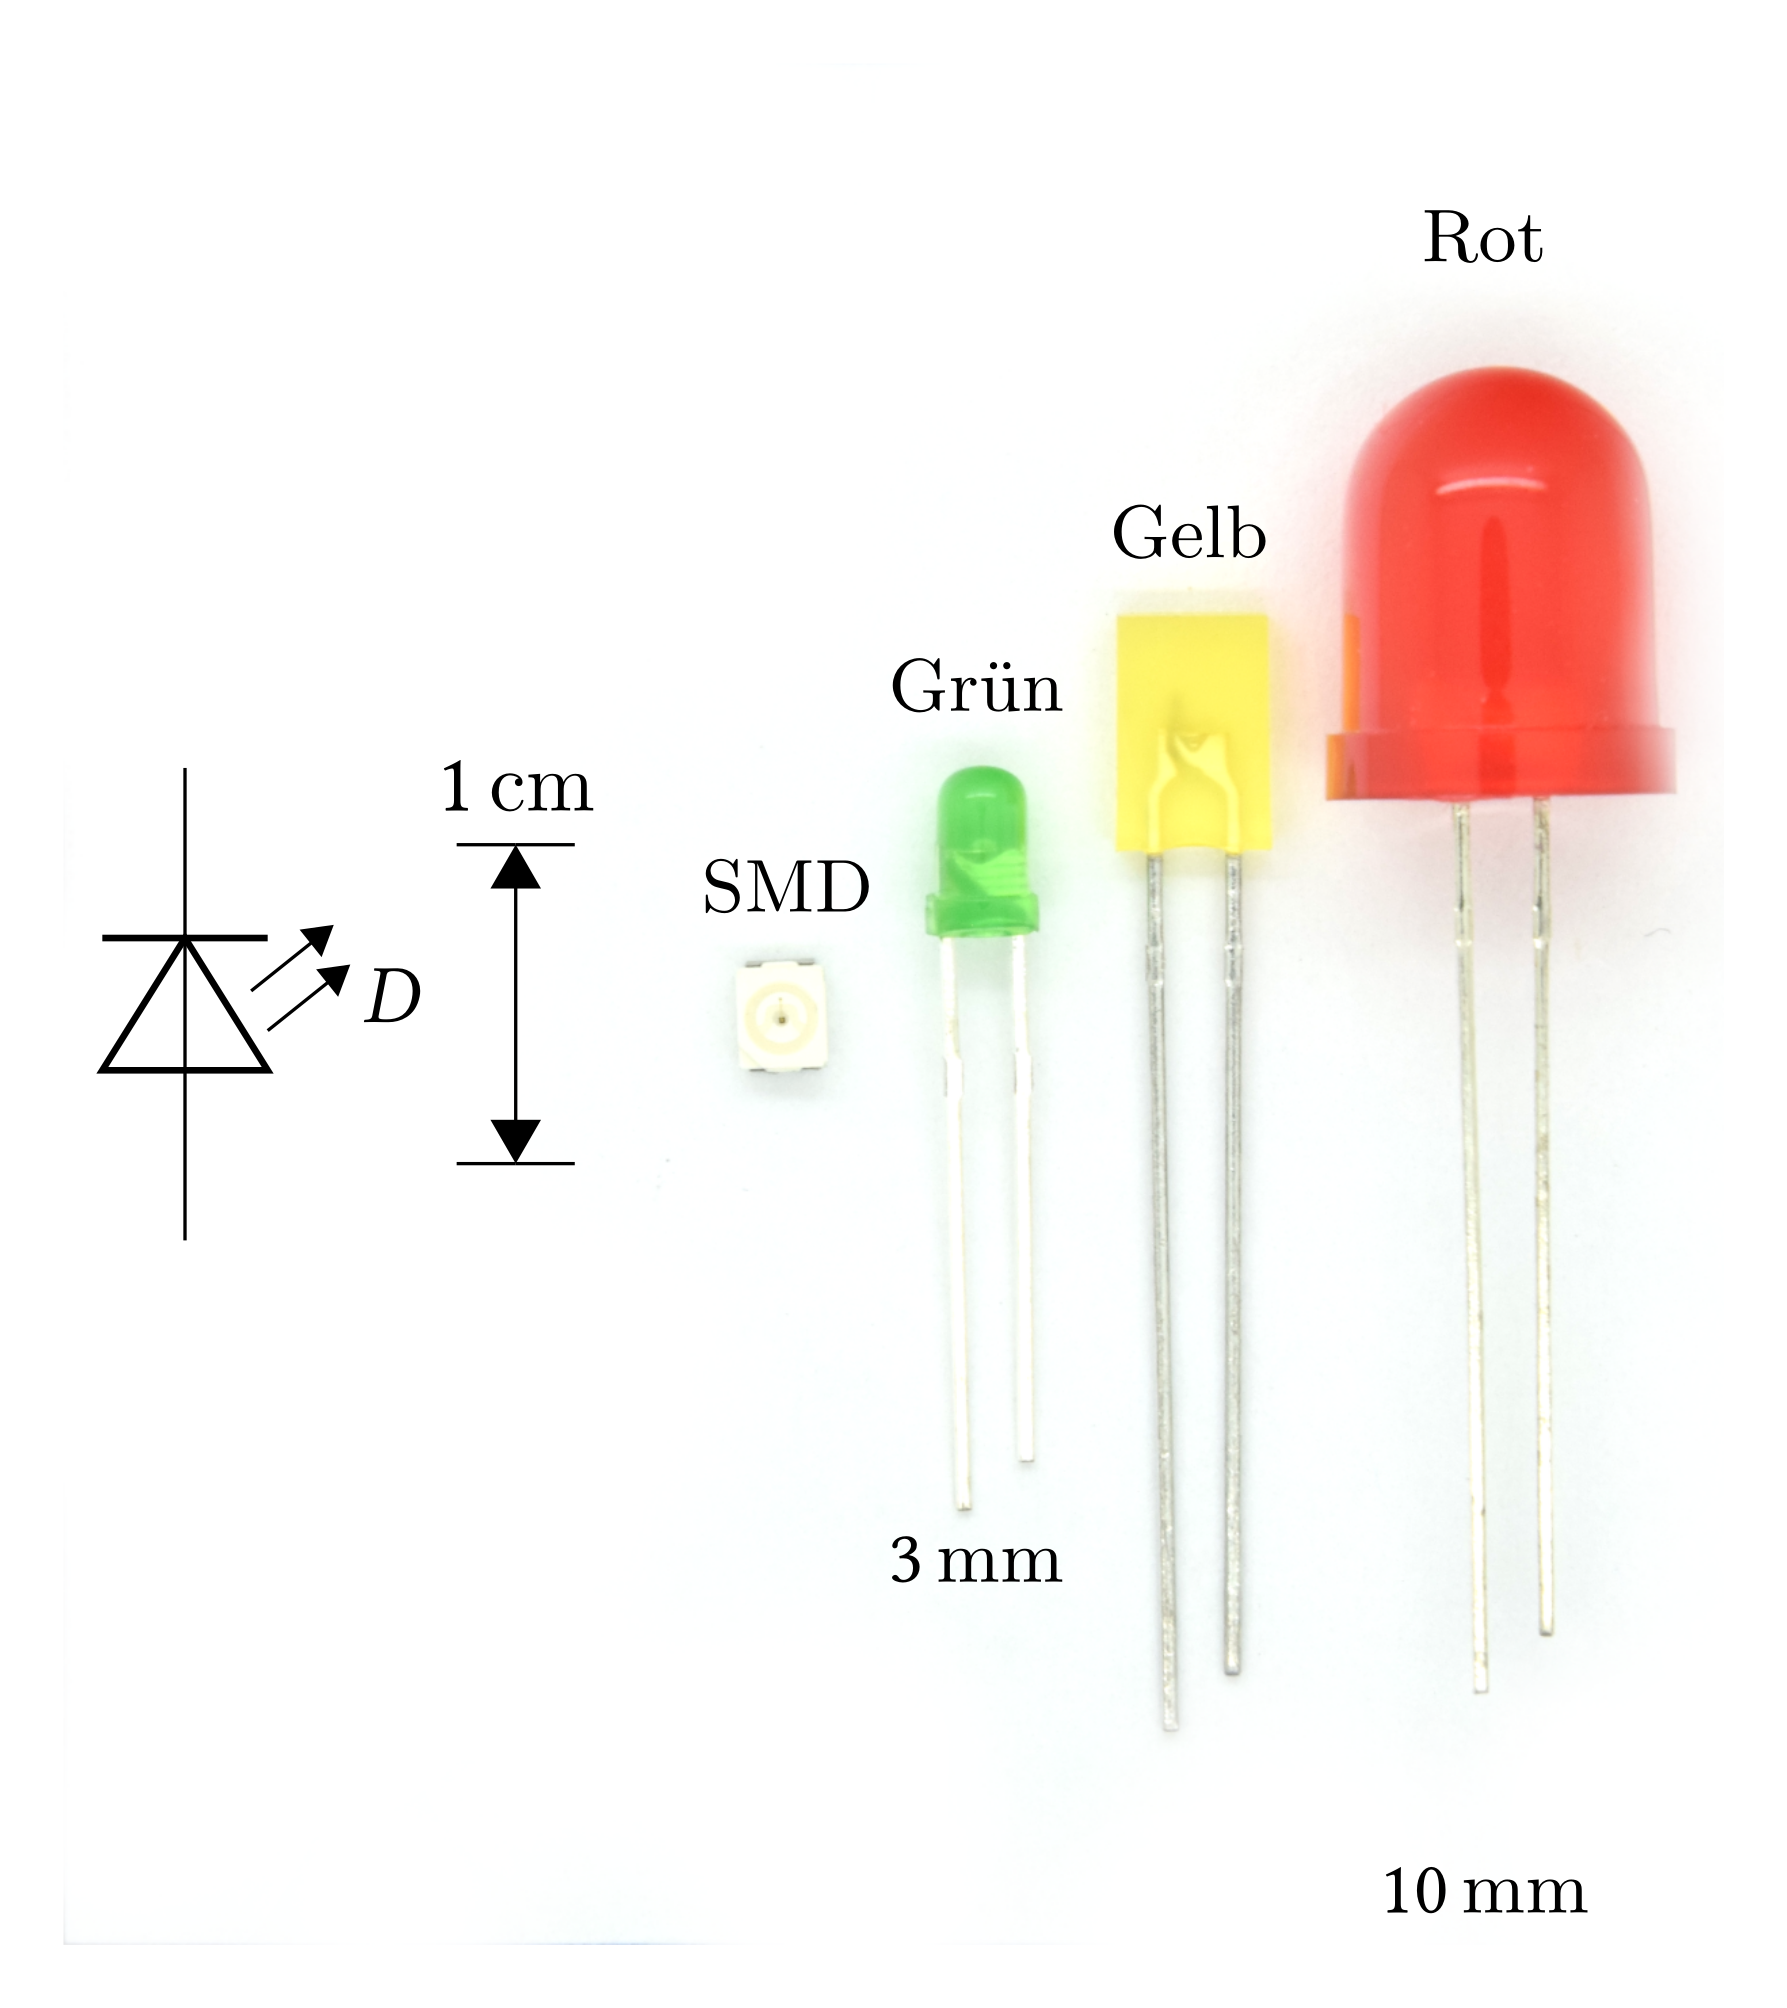
\includegraphics[width=0.85\textwidth]{foto/205}
    \caption{\scriptsize Schaltzeichen und Bauformen von LEDs}
    \label{n_halbleiter_led}
\end{figure}

   \end{column}
\end{columns}

\end{frame}

\begin{frame}
\only<1>{
\begin{PQuestion}{NC402}{Welches Bauteil wird durch das Schaltzeichen symbolisiert?}{Batterie}
{Spule}
{Kondensator}
{Leuchtdiode}
{\DARCimage{0.5\linewidth}{522include}}\end{PQuestion}

}
\only<2>{
\begin{PQuestion}{NC402}{Welches Bauteil wird durch das Schaltzeichen symbolisiert?}{Batterie}
{Spule}
{Kondensator}
{\textbf{\textcolor{DARCgreen}{Leuchtdiode}}}
{\DARCimage{0.5\linewidth}{522include}}\end{PQuestion}

}
\end{frame}

\begin{frame}
\only<1>{
\begin{question2x2}{NB703}{Bei welchem der abgebildeten Stromkreise leuchtet die LED?}{\DARCimage{0.75\linewidth}{513include}}
{\DARCimage{0.75\linewidth}{514include}}
{\DARCimage{0.75\linewidth}{515include}}
{\DARCimage{0.75\linewidth}{516include}}
\end{question2x2}

}
\only<2>{
\begin{question2x2}{NB703}{Bei welchem der abgebildeten Stromkreise leuchtet die LED?}{\textbf{\textcolor{DARCgreen}{\DARCimage{0.75\linewidth}{513include}}}}
{\DARCimage{0.75\linewidth}{514include}}
{\DARCimage{0.75\linewidth}{515include}}
{\DARCimage{0.75\linewidth}{516include}}
\end{question2x2}

}
\end{frame}%ENDCONTENT
